% !TEX root = ../SegwayDoku.tex
\renewcommand{\autoren}{Stephan Morongowski}
\newpage
\subsection{Eigenbau eines Motortreibers}
Aufgrund der schlechten Verfügbarkeit eines zur feldorientierten Regelung von Synchronmotoren geeigneten Motortreibers wurde überlegt, einen solchen Treiber innerhalb der Projektarbeit zu entwickeln und zu bauen. Zur Eruierung des zeitlichen und kostenmäßigen Aufwandes wurden zunächst grobe Anforderungen festeglegt und anschließend eine Marktrecherche sowie eine Machbarkeitsstudie durchgeführt.

\subsubsection{Anforderungen an den zu entwickelnden Treiber}
Eine Skizze zur prinzipiellen Anordnung der nötigen Komponenten ist in Abbildung \ref{kompVec} gegeben.

\begin{figure}[h]  % [h] bedeutet, dass das Bild genau an dieser Stelle im Text erscheint
\centering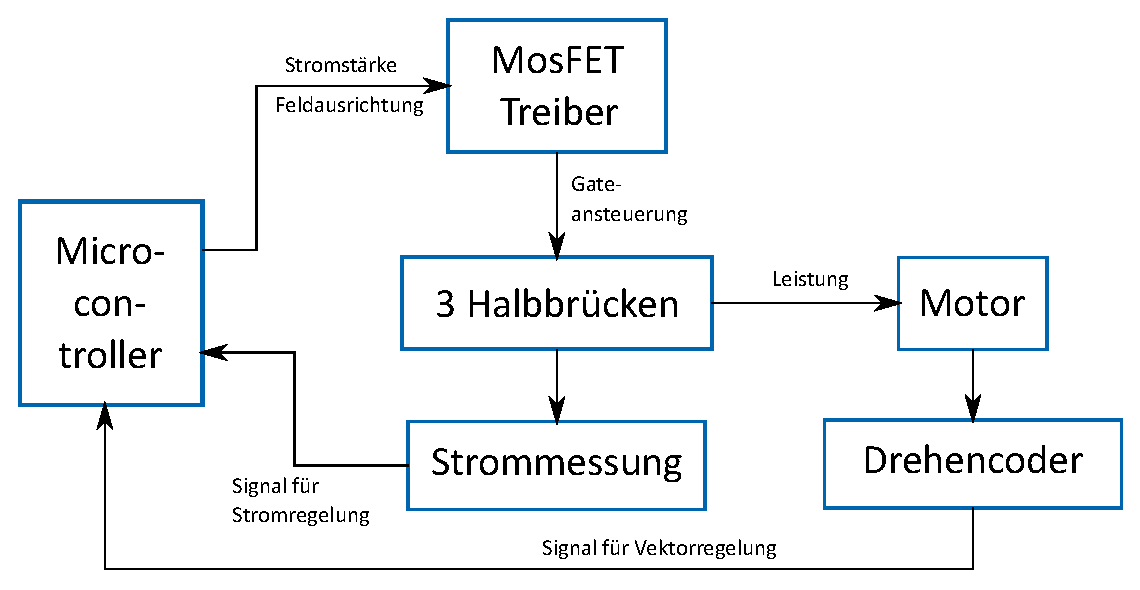
\includegraphics[width=0.8\textwidth]{images/KomponentenVektorregelung.eps}
\caption{notwendige Komponenten eines potentiellen Motortreibers \newline (Quelle: eigene Darstellung, SM)}
\label{kompVec}
\end{figure}

\begin{benannteAuflistung}[Notwendige Komponenten für zwei Motoren:]
    Microcontroller & 12-24 Pwm-Ausgänge pro Motor bei min. 20kHz \\
    & 4-6 digitale Eingänge für Quadraturencoder \\
    & 4 digitale Eingänge für Sollmomentvorgabe (Moment und Richtung) \\
    & 4 analoge Eingänge für Strommessung pro Motor \\
    Leisungstransistoren & 6 Halbbrücken (High-Side-Ansteuerung über Ladepumpe oder Pull-Up Widerstand zur Motorversorgungsspanung)  \\
    Sensorik & 4 mal Strommessung \\
\end{benannteAuflistung}

\par\bigskip

\begin{benannteAuflistung}[Gewünschte Technische Daten:]
    Motorspannung & bis 25V \\
    Strom & dauerhaft 30A, Spitze 50A \\
    Schnittstellen & I2C, USB, PWM \\
\end{benannteAuflistung}

\par\bigskip

Die Herstellungskosten sollten XXX,- € nicht übersteigen.

\par\bigskip



\subsubsection{Marktanalyse}

\subsubsubsection{VESC}
\label{sssec:vesc}
Der VESC - vector electronic speed control \cite{vesc} ist ein openSource Projekt von Benjamin Vedder. Der Treiber wurde ausgelegt, um ein Skateboard mit einem bürstenlosen Gleichstrommotor anzutreiben und ist in der Lage, 240A Spitzenstrom und 50A Dauerstrom bei bis zu 60V Versorgungsspannung zu liefern. Er verfügt über eine umfangreiche Konfigurationssoftware, über die vom PC aus alle nötigen Voreinstellungen vorgenommen werden können. Das ganze Projekt wirkt auf den ersten Eindruck sehr ausgereift.


\par\bigskip
\begin{benannteAuflistung}[Technische Daten:]
    Microcontroller & STM34F4 \\
    MOSFET Treiber & DRV8302 \\
    MOSFETS & 6 IRFS7530 \\
    Motorspannung & 8V - 60V \\
    Strom & dauerhaft 50A, Spitze 240A \\
    Schnittstellen & PPM signal (RC servo), analog, UART, I2C, USB, CAN-Bus \\
    Größe & 40mm mal 60mm \\
\end{benannteAuflistung}

\par\bigskip


\begin{benannteAuflistung}[Kosten im Eigenbau für zwei Stück:]
    Bauteile & ca. 120,- € \\
    Platinen & ca. 100,- €\\
    Lötzubehör & ca. 20,- € \\
    \textbf{Summe} & \textbf{ca. 240,- €} \\
\end{benannteAuflistung}

\par\bigskip
Beschaffungskosten für zwei fertig aufgebaute Platinen: \textbf{ca. 280,-€}

\newpage
\subsubsubsection{ODrive}
\label{sssec:odrive}
Der ODrive ist eine Entwicklung verschiedener Personen, da grundsätzlich jeder an der Entwicklung des Treibers teilnehmen kann. Dieser Treiber steuert bis zu zwei Motoren mit je ca. 100A Spitzenstrom. Das Projekt befindet sich noch in der Entwicklungsphase. Die Konfiguration des Treibers muss in die Firmware kompiliert werden.

\par\bigskip




\par\bigskip
\begin{benannteAuflistung}[Technische Daten:]
    Microcontroller & STM34F4 \\
    MOSFET Treiber & DRV8301 \\
    MOSFETS & 28 NTMFS4935NT1G \\
    Motorspannung & 8V - 30V \\
    Strom & dauerhaft ?, Spitze > 100A \\
    Schnittstellen & USB, CAN, UART, PWM, and step/dir interface \\
    Größe & 110mm mal 50mm \\
\end{benannteAuflistung}


\par\bigskip



\begin{benannteAuflistung}[Kosten im Eigenbau pro Stück:]
    Bauteile & ca. ???,- € \\
    Platinen & ca. ???,- €\\
    Lötzubehör & ca. 20,- € \\
    \textbf{Summe} & \textbf{ca. ???,- €} \\
\end{benannteAuflistung}

\par\bigskip
Beschaffungskosten als fertig aufgebaute Platine: \textbf{ca. 120,-€}

\subsubsubsection{Predriver}
Zur effizienteren Nutzung der MosFET wird von verschiedenen Herstellern ein Predriver angeboten. Zur Verfügung steht z.B. der DRV8305 von TI. Er stellt als Funktionen die nötige Ladepumpe, eine Möglichkeit zur Strommessung, optimierte Schaltung der FETs und andere Funktionen zur Verfügung.

\subsubsubsection{fertige Halbbrücke als Smd-Bauteil}
Infineon hat fertige Halbbrücken im Programm, die einige der benötigten Anforderungen bereits ohne externe Komponenten erfüllen. Als Beispiel sei hier der BTN8962TA vorgestellt:

\par\bigskip
\begin{benannteAuflistung}[BTN8962TA]
    Strom & dauerhaft 30A, Spitze 70A \\
    Spannung & bis 40V \\
	Ladepumpe & integriert \\
	Strommessung & integriert \\
	PWM & bis 25kHz \\
	Ansteuerung & logic level \\
	benötigte Menge & 6 Stück \\
	Einzelpreis & ca. 4,22€ \\
	\textbf{Gesamtkosten} & \textbf{ca. 25,-€} \\
\end{benannteAuflistung}

\subsubsubsection{Aufbau der Halbbrücken aus Einzelkompoenten}
\begin{benannteAuflistung}[Benötigte Komponenten][llX]
    MosFETs & 6 n-FETs  & ca. 3,-€ \\
	& 6 p-FETs & ca. 3,-€ \\
	Predriver & zB & ca. 5,-€ \\
	Strommessung & 4 Shuntwiderstände & ca. 3,-€ \\
	\textbf{Gesamtkosten} & & \textbf{ca. 14,-€} \\
\end{benannteAuflistung}

\subsubsubsection{Auswahl eines Microcontrollers}
\begin{benannteAuflistung}[Benötigte Eigenschaften pro Motor]
    6 Pwm-Ausgänge pro Motor bei min. 20kHz \\
    6 digitale Ausgänge pro Motor \\
    2-3 digitale Eingänge für Quadraturencoder \\
    2 digitale Eingänge für Sollmomentvorgabe (Moment und Richtung) \\
    2 analoge Eingänge für Strommessung pro Motor \\
\end{benannteAuflistung}
\par\bigskip

Zusätzlich zu den o.g. Angaben muss der Controller gut programmierbar sein und sollte keine, für die Projekt- und Labormitarbeiter völlig neuartige, Programmierumgebung darstellen. Auf Grund dieser Vorgabe wird die Auswahl eingeschränkt auf Controller, die entweder von dem Arduino-Framework oder dem mbed-Framework unterstützt werden. 
\par \smallskip
\begin{benannteAuflistung}[mögliche Kanditaten]
    Atmega 1280 & ca. 9,-€ \\
    Atmega 2560 & ca. 10,-€ \\
    STM32F4 & ca. 9,-€ \\
    STM32F7 & ca. 10,-€ \\
\end{benannteAuflistung}
\par\smallskip
Die Controller von Atmel liegen bei gleichem Preis in ihrer Leistung deutlich unter der Leistung der Controller von ST.

\subsubsubsection{Komplettlösungen als integrierter Schaltkreis}
Auf dem Markt finden sich verschiedene Ein-Chip-Lösungen für den Betrieb eines Synchronmotors. Jedoch sind diese in der Regel für sensorlosen Antrieb ausgelegt und damit im Stillstand nicht gut betreibbar. Des Weiteren liegen die erreichbaren Ströme weit unter den Projektanforderungen.

\subsubsection{Fazit}
Der Ankauf fertiger Motortreiber ist zu teuer. Ein eigenständiger Nachbau der Controller Vesc (siehe \ref{sssec:vesc}) oder ODrive (siehe \ref{sssec:odrive}) wird in etwa die gleichen Kosten produzieren, wie die Anschaffung der fertig bestückten Platinen und zusätzliche Arbeit schaffen.
Andere fertige Lösungen stehen derzeit nicht zur Verfügung.\\
 Es erscheint demnach am Sinnvollsten, einen an die Projektanforderungen angepassten Controller im Eigenbau neu zu entwerfen.


\newpage
